\chapter[From Parton Model to TMDs]{From Parton Model to TMDs}
In this chapter, I will explore the basic assumptions of the parton model and construct the definition of transverse-momentum-dependent parton distribution functions (TMD PDFs), which are the physical quantities we aim to infer from experimental data.

\subsection[QCD Lagrangian and Asymptotic Freedom ]{QCD Lagrangian and Asymptotic Freedom}
Hadrons, such as protons, are are composed of partons, quarks and gluons, which are in a confined state at our energy scale. The interactions between quarks and gluons are described by quantum chromodynamics (QCD) \cite{Peskin:1995ev}, a Yang-Mills theory that promote global $SU(3)$ invariance to a local invariance (\textit{i.e.} the QCD Lagrangian is invariant under local color transformation). Here, I present the QCD Lagrangian, including only one quark of mass $m$ and excluding ghost fields for simplicity \cite{Grinstein:2003zz} :

\begin{equation}
\label{eq:lagrangian_QCD}
 \mathcal{L} = - \frac{1}{4} F_{\mu \nu}^aF^{a \mu \nu} + \bar{\psi}^i(i \slashed{D}_j^k - m\delta_j^k)\psi_k
\end{equation}

Where $a = 1, 2, ..., 8$ is the color index; $\psi \text{, }\bar{\psi}$ represent the fermion fields (quarks). The gauge-fields $A_{\mu}^a$ (gluons) are enclosed in the gauge-field strength tensor 

\begin{equation}
\label{eq:gluon-strength_tensor}
F_{\mu \nu}^a = \partial_\mu A_\nu^a - \partial_\nu A_\mu^a + g f^{abc} A_\mu^b A_\nu^c
\end{equation}

and in the covariant derivative 

\begin{equation}
\label{eq:covariant_derivative}
\slashed{D} = \gamma^{\mu} D_{\mu}  = \gamma^{\mu}(\partial_{\mu} - igA_{\mu}^a T^a)
\end{equation}

If we expand all terms of the Lagrangian we obtain the strong interaction terms:

\begin{equation}
\label{eq:lagrangian_interactions}
\mathcal{L} = \mathcal{L}_0 + g A_{\mu}^a \bar{\psi}\gamma^{\mu}T^a \psi + g f^{abc}(\partial_{\mu}A_{\nu}^a)A^{b\mu}A^{c\nu} - g^2  f^{eab}  f^{ecd} A_{\mu}^a A_{\nu}^b A^{c \mu} A^{d \nu}
\end{equation}

It is interesting to note that all the terms in equation \eqref{eq:lagrangian_interactions} represent different types of interaction. The first term is the non-interacting contribution, the second term represent the interaction between two leptonic fields and a gluon, and the third and fourth terms represent the interactions between three and four gluon fields, respectively. All these terms are weighted by powers of the gauge coupling $g$. \\

From the QCD Lagrangian, we can deduce the Feynman rules for calculating amplitudes of elementary processes involving quarks and gluons in terms of the strong coupling, $\alpha_s = \frac{g^2}{4\pi}$. If $\alpha_s$ were a small constant, we would have some dominant processes (those with a small number of vertices) and some negligible higher order contribution, similar to the case of quantum electrodynamics (QED) where the amplitude of processes get smaller with an increasing number of vertices in the corresponding Feynman diagram. Unfortunately, the strong coupling is small only at high energy scales preventing us from developing a fully perturbative approach. This phenomenon is known as asymptotic freedom, the strong coupling $\alpha_s$  depends on the energy scale~\eqref{eq:alpha_strong}. At high energy (short distance interactions) the strong coupling becomes very small. As the particles get closer to each other they become more free, but as the distance increases (or, equivalently, the energy decreases), the strong coupling $\alpha_s$ increases. 

\begin{equation}
\label{eq:alpha_strong}
\alpha_s(Q) = \alpha_s (\mu)\frac{1}{1+\frac{b_0  \alpha_s (\mu) \ln(\frac{Q}{\mu})}{2\pi}}
\end{equation}

If we consider the coupling running towards smaller energies, we can rewrite the previous expression as follows: 

\begin{equation}
\label{eq:alpha_strong2}
\alpha_s(Q) =\frac{1}{b_0  \ln(\frac{Q}{\Lambda})}
\end{equation}

for energies below $1 GeV$ the strong coupling diverges rapidly, with a pole at $\Lambda \propto 200 MeV$, causing the confinement of quarks.

Asymptotic freedom is crucial for describing hadronic interactions, because it ensure us that we can use a perturbative approach to compute the amplitude of short range processes order by order. However, for a complete description of hadronic interactions we cannot consider only short distance interactions; we need to introduce some non-perturbative functions to parametrize that part of the process that we do not know how to predict. This approach was first introduced in the parton model, which is the argument of the next paragraph.


\subsection[The Parton Model]{The Parton Model}
Historically, the parton model was introduced before the theory of QCD to explain the results of the SLAC-MIT experiment~\cite{Taylor:2000dg}, in which electrons and protons were scattered at energies up to $20 GeV$. This scattering experiment lead to the confirmation that the proton is not an elementary particle, instead it is composed by point-like particles, named partons by Feynman in 1968, these are the quarks of QCD. According to the parton model, introduced by Bjorken and Feynman, when an electron interacts with a proton at high energy, the interaction occur between the electron and one of the proton fundamental constituents, which carries a fraction $\xi$ of the total momentum of the proton. After the parton-electron interaction, the struck quark interacts with the other partons on a much larger time scale and the proton breaks up.

To explain the basic assumptions of the parton model, I will consider a process of Deep Inelastic Scattering (DIS, $\ell(k) p(P)  \to \ell(k') X$), in which an high energy electron scatters off a proton target (Figure~\ref{fig:DIS}).

\begin{figure}[htbp]
\begin{center}
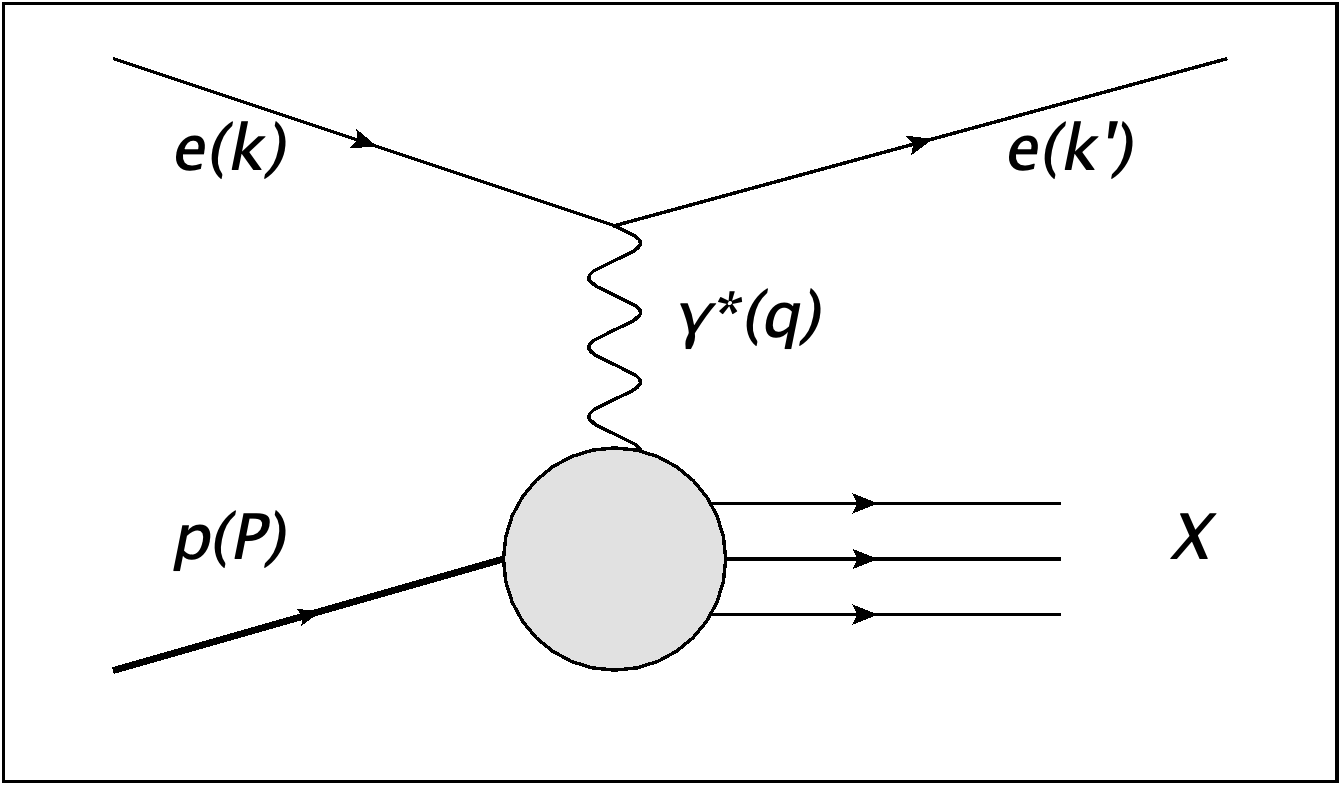
\includegraphics[width=\textwidth]{Images/chapter1/DIS.png}
\caption{DIS $\ell(k) p(P)  \to \ell(k') X$}
\label{fig:DIS}
\end{center}
\end{figure}

We can make some heuristic assumptions for this process:
\begin{enumerate}
\item the proton is composed by a collection of point-like particles (partons)
\item the partons move all in the same direction, longitudinal to the moving direction of the proton. This is of course an approximation, we neglect the transverse components because, in the center of mass reference system, the proton is moving at high speed along only one axis
\item each parton carries a fraction $\xi$ of the longitudinal momentum of the proton $P$, the longitudinal momentum of the parton will be $p = \xi P$
\item the partons are free particles (they do not interact with each other), the interaction occur between the electron $e$ and one single parton $q_i$: $e(k) q_i(p) \to e(k') q_i(p')$
\end{enumerate}

The last assumption is crucial, but is hard to believe. As we know, the interaction between two quarks (strong interaction) should be much stronger than the interaction between a quark and an electron (electromagnetic interaction), how come that we can approximate partons as free particles? The answer comes from QCD and asymptotic freedom: when we consider an high energy interaction (with large transverse momentum of the final state particles), we are in an energy region in which the strong coupling is weak, and the electromagnetic interaction dominates. A more intuitive argument can be given to justify the assumption that quarks are free particles \cite{CTEQ:1994ydo} \cite{Collins:2003fm}: we consider the time scale of the interaction binding two quarks to be $\tau_1 \propto 1 \frac{fm}{c}$ and the time scale of the quark-electron interaction at energy $Q$ to be $\tau_2 \propto \frac{1}{Qc}$. In the center of mass frame the time $\tau_1$ dilates and becomes $\tau_1' = \tau_1(1-\frac{v^2}{c^2}) >> \tau_1$. As an example, if we take an event at $\sqrt{s} = 300 GeV$ we get $\tau_1' \propto 100 \frac{fm}{c}$ and $\tau_2 \propto 0.01\frac{fm}{c}$. It is therefore a reasonable approximation, in the time scale of the parton-electron interaction, to treat the quarks as 'frozen' states with a momentum of $p=\xi P$. \\

Using these assumptions, one can reconstruct the elementary cross section, $$\hat{\sigma}(e(k)q_i(p) \to e(k') q_i(p')$$ order by order in perturbative QCD; for example, the tree level elementary cross section will be the same as the cross section for the leptonic process $e(k) \mu(p) \to e(k') \mu(p')$, with the only difference that the considered quark $q_i$ has a different charge than the muon $\mu$.

\subsubsection{Deep Inelastic Scattering Kinematics}
To define the DIS cross section, we have to define the kinematics of the process in figure~\ref{fig:DIS}. Consider the electron-proton collision $$e(k)p(P) \to e(k') X$$ in which $X$ represent an hadronic final state that is not measured. We can define two Lorentz invariant quantities: $Q^2 = t = (-q)^2$ and $P \dot q$, where $P$ is the momentum of the initial state proton and $q = (k-k')$ is the space like exchanged momentum. Two useful combination of these quantities are 

\begin{align}
x_B &= \frac{Q^2}{2Pq} \\
y     &= \frac{qP}{kP}
\end{align}

$x_B$ is the Bjorken variable and represents the fraction of the total momentum carried from the struck parton, $x_B=\xi = \frac{p}{P}$, $y$ represents the fraction of energy lost by the electron during the interaction, $\frac{E-E'}{E}$. Both variables lie between $0$ and $1$ and can be expressed in terms of the measurable quantities $k$, $k'$ and $P$. We have now all the ingredients to construct the hadronic cross section for deep inelastic scattering.

\subsubsection[DIS cross section]{DIS Cross Section}
We are able to compute with high precision the elementary cross section $\hat{\sigma}(e(k)q_i(p) \to e(k') q_i(p'))$, but we can not directly measure this short-range interaction, that means we do not know with which parton the electron interacts and neither we know the internal momentum distribution of the hadron. To address this problem we introduce the parton distribution functions (PDFs) $f_i(x)$. This function represents the probability that the i-th parton carries a fraction x of the total longitudinal momentum and is the link between the measured cross section and the elementary process (equation~\eqref{collinear_PDF}).

\begin{equation}
\label{collinear_PDF}
\frac{d \sigma}{dt}(e(k)p(P) \to e(k') X) =\sum_i \int dx f_i(x) \frac{d\hat{\sigma}}{dt}(e(k)q_i(p) \to e(k') q_i(p')) 
\end{equation}
  































